\documentclass{article}
\usepackage[utf8]{inputenc}
\usepackage{graphicx}

% change reference style to [1], remove stupid sorting, language changed so date in ddmmyyyy
\usepackage[backend=biber, style=numeric, sorting=none, language=australian]{biblatex}
\addbibresource{References.bib}

\title{Dissertation}
\author{David Saunders (910995)}
\date{September 2020}

\begin{document}
\maketitle

\begin{abstract} 
    Write abstract here
\end{abstract}

\tableofcontents

\section{Section 1}

This paper has a nice scientific explanation of n-grams \cite{tomovic2006n}.
Either cite this paper or more likely look at their reference for n-grams and cite that.

\section{Data Pipeline}

When planning and completing this project many decisions were made about the steps taken to convert the raw data to a finished product/classification.

\begin{figure}[ht]
    \centering
    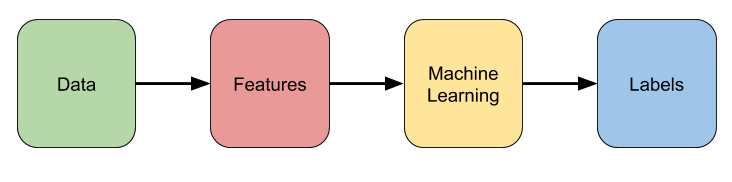
\includegraphics[scale=0.55]{Images/Data-Pipeline.png}
    \caption{Diagram of the Data pipeline of the project.}
    \label{fig:test}
\end{figure}

\subsection{Data}

Here I will summarise what I have done to the data.
As previously mentioned the data was gathered through a lab study and an online study.
The purpose of the online study was to gather a larger amount of data that was possible to do so in person.
The aim of this was to make any results more statically significant.

This leads to the problem of imbalanced data samples.
There were approximately 11 lab data and 400 online data, meaning that there were 40x as many data samples from one class compared to the other.
As stated in my assumptions, we can say that the lab participants were paying attention, where as the online participants may or may not have been paying attention.

If the classes were balanced then simple approach may be to treat this problem as binary classification problem.
Using something like a Support Vector Machine we could classify a given point as lab or online / paying attention or possibly paying attention based on their proximity to other data points.
To do so we would need to have balanced classes otherwise the algorithm would have a high accuracy from just classifying everything as possibly paying attention as that is the most frequent class.
There are two main methods of dealing with class imbalances, removing data samples and creating new data samples.

It was decided that creating new data samples would be best as there is not a whole lot of data to work with, so there would be a strong preference to keep the data we have.
New points can be created by sampling from a distribution (reference) but here it was decided just to duplicate the samples as there was no discernible distribution of the data.
Another method is to copy the points, altering them slightly, this was considered but not used in the end.
Each lab study data sample was copied 40 times to even out the classes.

\subsection{Features}



\printbibliography

\end{document}